\section{Teknologier til smerteklassificering} % Anden overskrift...
\textit{I denne sektion vil nuværende teknologier til undersøgelse af neural aktivitet blive beskrevet med særlig fokus på anvendelse i forbindelse med undersøgelse af smerteopfattelse. Det økonomiske aspekt vil ligeledes blive analyseret for de enkelte teknologier. Afslutningsvis vil der blive foretaget en sammenligning med henblik på at identificere fordele og ulemper ved de enkelte teknologier.}

For at understøtte klinikerens vurdering af de enkelte patienter vedrørende henstilling til TKA, kan det overvejes, hvorvidt det vil være hensigtsmæssigt at tilføje en ekstra undersøgelse til patientens udredningsforløb forud for beslutningstagen. Relevante undersøgelser kan eksempelvis være objektive målinger af neural aktivitet i forskellige situationer, samt vurdering af patienternes individuelle respons på forskellige typer af stimuli. 

%Til undersøgelse af aktivitet i encephalon og nervesystemets funktion generelt findes flere forskellige metoder.

\subsection{Functional Magnetic Resonance Imaging}
Functional Magnetic Resonance Imaging(fMRI) er en metode til at undersøge aktiviteten i neuronerne i hjernen.
Generelt er MRI en metode til at synliggøre protoner; dermed er det muligt at afbilde kroppens væv, da dette primært er udgjort af hydrogen-atomer, som indeholder netop én proton.     
Ved en MRI-scanning udsættes objektet, eksempelvis en patient, for et eksternt magnetfelt, hvilket medfører, at der opstår et parallelt magnetfelt i objektet. Dermed er det muligt at detektere de tilstedeværende protoner, da deres retning skaber det parallelle magnetfelt i kroppen. \citep{Wals2009} Udgifterne til fMRI omfatter blandt andet indkøb af MR-scanner samt anvendelse og vedligehold. Prisen for en MR-scanner ligger mellem 1 og 8 millioner kr. \citep{Glover2014} \textbf{Note: Her bliver tilføjet mere økonomi specifikt}\fxnote{Er i tvivl om, om dette er nok, men ellers er man nødt til at anvende sider, der sælger MR-scannere, og det er ikke særligt gode kilder... Alternativt kan der sættes ét priseksempel ind på en konkret scanner? + hvad det koster at lave en scanning feks på aauh} 
Der findes forskellige teknikker til fMRI, hvoraf de fleste anvender Blood Oxygenation Level-Dependent(BOLD) kontrast. Ved anvendelse af denne kontrast, udnyttes det, at der ved aktivitet i hjernens forskellige områder, vil ske en ændring af mængden af ilt i blodet, hvilket påvirker magnetfeltets styrke. Dermed vil det, ved hjælp af kontrastvæsken, være muligt at følge blodgennemstrømningens styrke i hjernens forskellige områder, og dermed belyse områder med øget aktivitet. \citep{Wals2009} 

\subsubsection{Anvendelse til detektion af smerte}
fMRI har i flere studier været anvendt til at undersøge neural aktivitet i forbindelse med knæsmerter.
I et studie af \citep{Parks2012} er det ved hjælp af fMRI blevet undersøgt, hvorvidt der er forskel på oplevelsen af kroniske smerter hos patienter med artrose og på smerter fremkaldt med tryk. Forsøgsdeltagerne var opdelt i en gruppe patienter med artrose i knæet og en gruppe raske individer. \cite{Parks2012} viste at de to grupper oplevede den kunstigt fremkaldte knæsmerte ens; der forekom stort set ingen variationer imellem de to grupper. Hos artrosepatienterne forekom der forskel i oplevelsen af de kroniske og de kunstigt fremkaldte smerter. \citep{Parks2012} 
I et andet studie af \cite{Hiramatsu2014} er det undersøgt, hvilke forskelle der forekom i cerebral respons hos en gruppe raske forsøgspersoner og en gruppe forsøgspersoner med kroniske knæsmerter forårsaget af artrose. Begge grupper blev udsat for akut smerte i knæet gennem invasive elektroder imens der blev foretaget en fMRI scanning. Studiet viste, at der hos gruppen af patienter med kroniske knæsmerter forekom en højere aktivitet i det dorsolaterale præfrontale cortex end hos gruppen af raske forsøgspersoner. \citep{Hiramatsu2014} 
fMRI kan således påvise forskelle på hvordan smerte opleves af forskellige grupper af mennesker. \figref{fig:fMRI_result} illustrerer forskellen i neural aktivitet mellem patienterne og den raske forsøgsgruppe.
\begin{figure}[H] 
	\begin{center}
		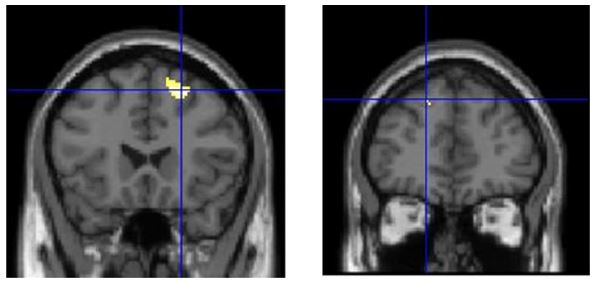
\includegraphics[width=0.7\textwidth]{figures/bProblemanalyse/fMRI_dorsolateral}
	\end{center}
	\caption{Figuren illustrerer forskellen imellem henholdsvis patientgruppen og den raske forsøgsgruppe. Det fremgår, at aktiviteten i det dorsolaterale cortex er signifikant højere hos patienterne end hos de raske individer. \citep{Hiramatsu2014}} 
	\label{fig:fMRI_result} 
\end{figure} 

\subsection{Quantitative sensory testing}
Quantitative sensory testing (QST) er en metode til undersøgelse af det sensoriske nervesystems funktion. Metoden kan anvendes til undersøgelse af forskellige egenskaber, herunder smertegrænser. QST eksponerer patienten for forskellig sensorisk sensation, herunder tests, der involverer varme og kulde, vibration og tryk. Dermed er det muligt at identificere grænserne for henholdsvis perception og smerte. \citep{Yarnitsky2006} Prisen for en maskine som kan anvendes til QST afhænger af hvilken QST protokol der anvendes. Firmaet Nocitech har udarbejdet en maskine som kan anvendes til at undersøge tre parametere med henblik på detektering af muskuloskeletale smerter. Denne maskine koster $\sim$200.000 kr. \citep{NociTech2016} QST kræver i modsætning til fMRI ikke scanning eller anden billeddiagnostisk undersøgelse. \\
Der findes forskellige protokoller til udførelsen af QST, afhængigt af hvad formålet er med undersøgelsen. De forskellige protokoller indeholder forskellige tests, hvilket er baseret på fokusområdet. Et eksempel er en QST-protokol udviklet af German Network on Neuropathic Pain til undersøgelse af neuropatisk smerte. Ved brug af denne model anvendes syv forskellige tests til at vurdere 13 parametre, herunder seks temperaturtests til detektion af grænser for perception og smerte, samt syv mekaniske tests til detektion af tilsvarende grænser, her med henholdsvis spidse og stumpe genstande. I forbindelse med udarbejdelse af modellen er der desuden lavet tests for at opstille referenceværdier, der tager højde for køn og alder. \citep{Rolke2006}  

\subsubsection{Anvendelse til detektion af smerte}
QST bliver i forskningsregi anvendt til undersøgelse af patienter der får udført TKA. I et studie af \citep{Martinez2007} er en anden QST-protokol anvendt til at undersøge 20 patienter med artrose i knæet før og efter en TKA. Formålet hermed var at identificere faktorer, der har indvirkning på udviklingen af postoperative smerter. QST blev udført en enkelt gang før operationen og fire gange efter operationen. Perioden fra operationen og til QST undersøgelserne var på henholdsvis en dag, fire dage, en måned og fire måneder efter operationen. Parametrene der blev undersøgt i QSTen var tærskelværdier for temperatur, mekanisk smerte og hvordan de enkelte patienter responderede på en eksponering for temperaturer over tærskelværdierne. Studiet fandt, at der forekommer en sammenhæng mellem periodiske smerter efter operationen og de patienter, der oplever hyperalgesi under eksponering for varme. \citep{Martinez2007} Der skal imidlertid tages højde for, at der er flere fejlkilder forbundet med QST, da nøjagtigheden i høj grad afhænger af både patientens og undersøgerens præcision under udførelsen af de enkelte tests. Det må således forventes, at der kan forekomme variationer mellem enkelte QST udført på den samme patient. \citep{Yarnitsky2006} Forskningen i QST er intensiveret de senere år, i et studie fra 2015 af \citer{Arendt-Nielsen2015}, der er baseret på reveves af 17 studier, fandt man med QST at perifer og central sensibilisering er et prominent fænomen ved led artrose. Der vil med udviklingen i QST, være muligt at prifileret patienter og øge forståelsen af smertemekanismerne ved ledsmerter. \citep{Arendt-Nielsen2015}

\subsection{Elektrofysiologiske undersøgelsesmetoder}
De elektrofysiologiske undersøgelsesmetoder dækker over tests, der kontrollerer elektrisk aktivitet i kroppens celler. I hviletilstand har et neuron en fast spænding over sin membran. Når dette membranpotentiale ændres som følge af ændringer i koncentrationen af natrium- og kaliumioner inden- og udenfor cellen, genereres et aktionspotentiale, som vandrer langs cellens akson og videre til de følgende neuroner. Dette kan detekteres ved anvendelse af invasive eller non-invasive elektroder. Til monitorering af neuronernes funktionalitet i encephalon anvendes elektroencephalografi (EEG) mens der til monitorering af neuronernes funktionalitet i resten af kroppen anvendes elektroneurografi (ENG). Prisen for et EEG system er $\sim$550.000 kr. \citep{Biosemi2016} For at en elektrofysiologisk undersøgelse kan anvendes til at stille en diagnose, skal resultaterne herfra understøttes af andre kliniske undersøgelser, herunder prøver og lægesamtaler. \citep{Robinson2008} 

\subsubsection{Anvendelse til detektion af smerte}
I et studie af \citep{Brown2013}, er EEG blevet anvendt til at undersøge, hvordan to patientgrupper med forskellige sygdomme opfatter smerte. I studiet indgik en gruppe af patienter med artrose og en gruppe patienter med sygdommen fibromyalgi, der forårsager muskel- og ledsmerter \citep{Brown2013}\citep{9}. Hos de to patientgrupper blev det undersøgt, hvordan encephalon genererer signal for henholdsvis en forventning om og en decideret udløst smerte. Disse data sammenlignes med en kontrolgruppe bestående af raske personer. Der blev foretaget to målinger for at undersøge aktiviteten under forventning om smerte samt en måling under påført smerte. For hver forsøgsperson blev det efter målingerne undersøgt, fra hvilken elektrode, der dektekteredes den højeste amplitude, hvormed denne og de otte nærmeste elektroder blev udvalgt til yderligere analyse og udregning af gennemsnitlig amplitude. De gennemsnitlige målinger for de tre forsøgsgrupper er illustreret i \figref{fig:EEG_gns}.
\begin{figure}[H] 
	\begin{center}
		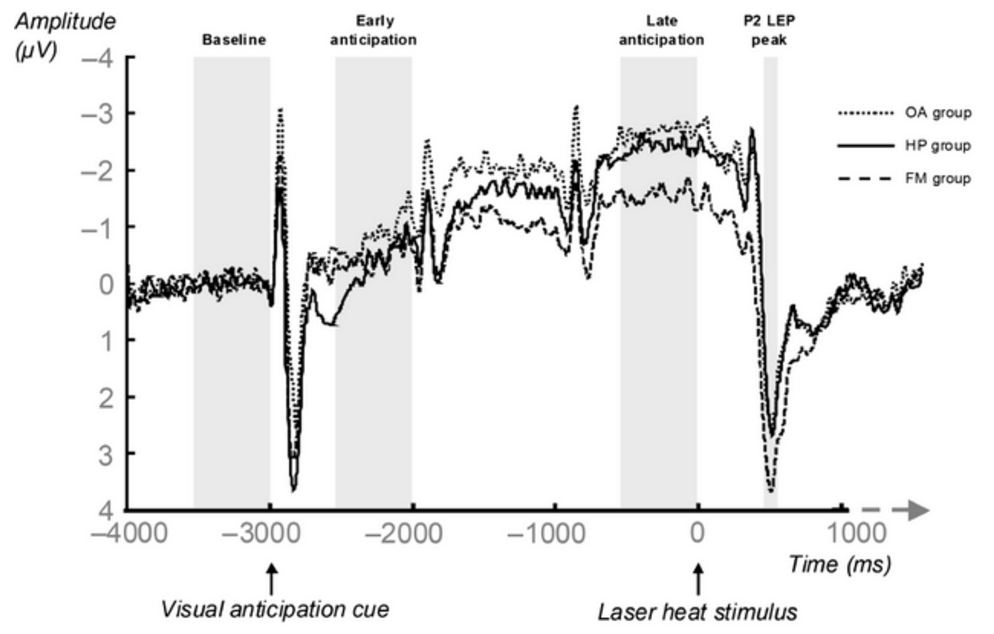
\includegraphics[width=0.7\textwidth]{figures/bProblemanalyse/EEG_ERP}
	\end{center}
	\caption{Figuren illustrerer de gennemsnitlige målinger for de tre forsøgsgrupper. Tidspunkter for måling af baseline, tidlig forventning, sen forventning og oplevelse af smerte er angivet på figuren. \citep{Brown2013}} 
	\label{fig:EEG_gns} 
\end{figure} 

Ud fra resultaterne var det muligt at undersøge i hvilke områder, der forekom særlig aktivitet ved hjælp af blandt andet billeddannende programmer. Resultaterne for studiet antyder, at de to patientgrupper responderer ens på forventningen om smerte, på trods af, at fibromyalgipatienternes respons var kraftigere. Disse resultater indikerer, at denne tendens kan være generelt gældende for patienter med kroniske smerter. \citep{Brown2013} Udgifterne til EEG-undersøgelse omfatter indkøb af udstyr samt løn til medarbejderne, der er med til at udføre undersøgelsen\citep{Green1985}.

\subsection{Vurdering af teknologier til smerteklassificering}
En optimal teknologi som vil kunne fungere som supplement til klinikerens beslutningstagen, vil skulle opfylde en bestemt række kriterier. Et af disse kriterier er at denne teknologi skal kunne anvendes til at klassificere smerte. Hvis ikke dette krav er opfyldt, vil teknologien ikke være anvendelig til at identificere patienterne i risikogruppen for at udvikle kroniske postoperative smerter, og vil heraf ikke kunne fungere som supplement. Teknologien bør tilmed være minimalt invasiv i afbenyttelse, hvoraf der bør opstå færrest mulige risici ved benyttelse. Ligeledes skal omkostningerne til anskaffelse af teknologien være mindst mulige, da dette vil være medvirkende til at teknologien vil være lettere organisatorisk implementerbar. \\
De analyserede teknologier er vurderet udfra ovenstående kriterier, og resultatet heraf ses i \tabref{tab:succeskriterier_metoder}  


\begin{table}[H]
	\centering
	\begin{tabular}{cccc}
		\hline
		\rowcolor[HTML]{C0C0C0} 
		Teknologi          & Klassificere smerte & Minimalt invasiv & Anskaffelsespris  {[}dkk{]} \\ \hline
		fMRI               & x                   & -                & 1 til 8 mio.          \\
		QST                & x                   & x                & 200.000               \\
		Elektrofysiologisk & x                   & (x)              & 550.00                \\ \hline
	\end{tabular}
	\caption{I tabellen ses hvilke kriterier de forskellige teknologier opfylder. Ved placering af ‘x’, indikeres det at kriteriet er opfyldt, men ved ‘(x)’ er kriteriet blot delvist opfyldt. Ved placering af ‘-’ er kriteriet ikke opfyldt.}
	\label{tab:succeskriterier_metoder}
\end{table} \vspace{-.5cm}
Alle de analyserede teknologier opfylder første kriterie vedrørende klassificering af smerte. Teknologierne opfylder ikke alle kravet vedrørende at skulle være minimalt invasiv. Dette medfører at fMRI bliver ekskluderet som en eventuel supplement til klinikerens beslutningstagen. fMRI kategoriseres som en invasiv teknologi, da patienten får injiceret kontraststoffet før denne metode kan anvendes til klassificering af patienten. QST opfylder kriteriet fuldt ud ved ikke at benytte invasive metoder til klassificeringen af smerte. Elektrofysiologiske metoder opfylder blot kriteriet delvist, hvilket er et resultat af at denne teknologi kan benytte både invasive og non-invasive elektroder til detektering af signalet, samt til dannelse af kunstig smerte gennem elektrisk stimulation. \\
I forhold til anskaffelsesprisen vil QST af de analyserede teknologier, være billigst. Ved implementering af QST skal teknologien indkøbes fra ny, hvilket er et resultat af det denne på nuværende tidspunkt blot benyttes i forskningsregi. MR-scannere og elektrofysiologiske metoder er allerede implementeret og bliver benyttet til anden diagnosticering og behandling. Resultatet heraf medfører at prisen for fMRI og de elektrofysiologiske metoder ikke er reel. Ved implementering af disse teknologier kan det antages at nyt udstyr ikke nødvendigvis bør indkøbes. Dog skal der tages forbehold at disse teknologier bliver anvendt andetsteds på hospitalet, hvormed der skal tages højde for længere ventetider for patienten end ved afbenyttelsen af QST. Dette kan antages da QST, som tidligere nævnt, ikke anvendes til diagnosticering af andre sygdomme. \\
Ud fra kriterierne og ovenstående overvejelser vil QST være den bedst egnede af de tre analyserede smerteklassificeringsmetoder som supplement til klinikerens udvælgelse af patienter til en TKA-operation.  



  
% 1 = fMRI techniques and protocols
% 2 = The dorsolateral prefrontal network is involved in pain perception in knee osteoarthritis patients
% 3 = Brain activity for chronic knee osteoarthritis: dissociating evoked pain from spontaneous pain
% 4 = Quantitative sensory testing
% 5 = The evolution of primary hyperalgesia in orthopedic surgery: Quantitative sensory testing and clinical evaluation before and after total knee arthroplasty
% 6 = Clinical electrophysiology
% 7 = When the brain expects pain: common neural responses to pain anticipation are related to clinical pain and distress in fibromyalgia and osteoarthritis 
%10 = Benefits, Shortcomings, and Costs of EEG Monitoring
%11 = http://time.com/money/2995166/why-does-mri-cost-so-much/ Glover2014
%12 = http://www.biosemi.com/faq/prices.htm Biosemi2016
%13 = http://nocitech.com/technology.html NociTech2016